\documentclass[10pt,a4paper]{article}
\usepackage{fontspec}
\setmainfont{Latin Modern Roman}
\setmonofont{Latin Modern Mono}
\usepackage[margin=2.2cm]{geometry}
\usepackage{amsmath,amssymb}
\usepackage{booktabs,multirow,array,tabularx,longtable}
\usepackage{graphicx,xcolor}
\usepackage{enumitem}
\usepackage{caption}
\usepackage{float}
\usepackage{tikz}
\usetikzlibrary{positioning,arrows.meta,fit}
\usepackage[hidelinks]{hyperref}
\usepackage{titlesec}

\titleformat{\section}{\Large\bfseries}{\thesection}{1em}{}
\titleformat{\subsection}{\large\bfseries}{\thesubsection}{1em}{}
\captionsetup{font=small,labelfont=bf}
\captionsetup[table]{labelformat=empty}
\renewcommand{\figurename}{Hình}
\setlist{itemsep=2pt,topsep=3pt}
\renewcommand{\arraystretch}{1.15}
\newcommand{\src}[1]{\texttt{[#1]}}
\setlength{\parindent}{0pt}
\setlength{\parskip}{4pt}

\begin{document}

\begin{center}
{\LARGE\bfseries BÁO CÁO KỸ THUẬT: NHÁNH SPHERICAL\\[2pt] CẢI THIỆN BỘ PHÂN LOẠI KAC}\\[6pt]
{\large Spherical Branch for KAC in Prompt-based Class-Incremental Learning}\\[10pt]
{\bfseries Huỳnh Thị Nhã Trân -- Nhóm DPL302m}\\[4pt]
Ngày 30 tháng 10 năm 2026
\end{center}

\vspace{4pt}
\textbf{Tóm tắt.} Báo cáo này trình bày phần cải tiến bộ phân loại KAC (Kolmogorov--Arnold Classifier) trên nền APT (Additive Prompt Tuning, ViT-B/16) trong bài toán học liên tục tăng dần lớp, không lưu mẫu cũ và không biết task id khi suy luận. KAC học mỗi task bằng cross-entropy trong phạm vi task đó, nên logit của các task khác nhau không cùng mức nền. Khi lấy argmax trên toàn bộ lớp đã học, mô hình dễ chọn nhầm task. Mình bổ sung một \emph{nhánh Spherical}: đưa đặc trưng lên mặt cầu đơn vị, biểu diễn mỗi lớp bằng vài tâm (spherical k-means) và chấm điểm theo phân phối von Mises--Fisher (vMF). Điểm này được kết hợp với KAC theo hai cách: \texttt{fuse} và \texttt{hier}. Nhánh Spherical được thử trên năm nguồn đặc trưng: ViT-B/16 đóng băng, APT (stale), APT (refresh, chỉ để tham chiếu), Swin-B và Swin-T đóng băng. Trên tập Validation (3 seed), biến thể \texttt{fuse} với ViT-B/16 đóng băng tăng Last so với APT + KAC ở cả 4 dataset: $+1.07$ (CIFAR-100), $+8.95$ (CUB-200), $+1.96$ (Stanford Cars), $+0.56$ (ImageNet-R) điểm phần trăm. Đổi sang Swin-B cho kết quả cao hơn một chút nhưng chậm hơn khoảng 2 lần. Hai hướng phụ (hiệu chỉnh logit KAC và giảm chiều đặc trưng) không mang lại cải thiện rõ ràng. Tất cả số liệu trong báo cáo là trên tập Validation, chưa chạy tập Test.

\section{Quy Ước Thực Nghiệm và Định Danh}

\subsection{Giao thức thực nghiệm chung}
\begin{itemize}
  \item \textbf{Bài toán:} Học liên tục tăng dần lớp không lưu mẫu (exemplar-free class-incremental learning). Khi suy luận lấy argmax trên toàn bộ lớp đã học, \emph{không} dùng task id.
  \item \textbf{Cách chia task:} CIFAR-100: 10 task $\times$ 10 lớp. CUB-200 và ImageNet-R: 10 task $\times$ 20 lớp. Stanford Cars-196: task đầu 16 lớp, 9 task sau mỗi task 20 lớp.
  \item \textbf{Số seed:} 3 seed $\{0,1,2\}$, báo cáo trung bình $\pm$ độ lệch chuẩn mẫu. Thứ tự lớp của seed $s$ là \texttt{RandomState(s).permutation}.
  \item \textbf{Chỉ số đánh giá:} Last $A_T$ (độ chính xác trên mọi lớp đã học sau task cuối), Avg $A_{avg} = \frac{1}{T}\sum_{t=1}^{T} A_t$, và Forgetting (mức giảm trung bình so với độ chính xác cao nhất trước đó của mỗi task). Kết quả chính đọc theo \textbf{Last}.
\end{itemize}

\subsection{Quy chuẩn phân chia dữ liệu}
\begin{itemize}
  \item \src{Tập Validation}: Tập train gốc được chia stratified 5 fold theo lớp (\texttt{RandomState(1993)}). Với seed $s$, fold $s$ làm Val, 4 fold còn lại (80\%) dùng để huấn luyện. Toàn bộ số liệu trong báo cáo này thuộc giai đoạn Val.
  \item \src{Tập Test}: Chưa sử dụng. Test chỉ chạy một lần sau khi đã chốt cấu hình trên Val, để không rò rỉ thông tin từ tập kiểm thử.
  \item \textbf{Chọn cấu hình:} Với mỗi dataset, nguồn đặc trưng và biến thể, mình chọn bộ siêu tham số có Last trung bình 3 seed cao nhất trên Val (lưới ở Mục~\ref{sec:method}).
\end{itemize}

\subsection{Tiền tố nguồn gốc số liệu}
\begin{itemize}
  \item \src{Baseline}: APT + KAC do nhóm chạy bằng repo APT chính thức, thay đầu phân loại bằng KAC (4 lưới RBF, lr head $10^{-3}$). Siêu tham số APT lấy từ \texttt{experiments/*.sh} của repo: batch 64, \texttt{prompt\_param} 0.01; CUB lr 0.02, 25 epoch, EMA 0.7.
  \item \src{Ours}: APT + KAC kết hợp nhánh Spherical (cùng split, cùng seed với Baseline).
  \item \src{Tham chiếu}: Cấu hình cần truy cập lại ảnh của task cũ, nên không hợp lệ trong thiết lập không lưu mẫu. Chỉ dùng để ước lượng mức trần nếu khắc phục được drift của đặc trưng.
\end{itemize}

\subsection{Nguồn đặc trưng cho nhánh Spherical}
Nhánh KAC luôn giữ nguyên (APT + KAC). Chỉ đặc trưng đưa vào nhánh Spherical thay đổi:
\begin{itemize}
  \item \texttt{ViT-B/16 đóng băng}: ViT-B/16 tiền huấn luyện, không gắn prompt. Dùng chung trọng số với backbone của APT nên không thêm tham số, chỉ thêm một lượt forward không prompt.
  \item \texttt{APT (stale)}: Đặc trưng CLS sau prompt của APT. Tâm của một lớp được tính ngay sau task chứa lớp đó và không cập nhật lại. Ảnh test được nhúng bằng mô hình hiện tại. Đây là cấu hình hợp lệ, nhưng tâm cũ bị lệch khi prompt tiếp tục được cập nhật.
  \item \texttt{APT (refresh)} \src{Tham chiếu}: Ở mỗi bước, tính lại tâm của mọi lớp đã học bằng mô hình hiện tại trên ảnh train cũ.
  \item \texttt{Swin-B / Swin-T đóng băng}: Backbone riêng (\texttt{swin\_base\_patch4\_window7\_224.ms\_in22k\_ft\_in1k}, 1024 chiều; \texttt{swin\_tiny\_patch4\_window7\_224.ms\_in1k}, 768 chiều), không huấn luyện.
\end{itemize}

\subsection{Quy ước gọi tên biến thể}
\begin{itemize}
  \item \texttt{fuse}: Trộn log-xác suất của KAC và Spherical trên toàn bộ lớp đã học (công thức~\eqref{eq:fuse}).
  \item \texttt{hier}: Spherical chọn task, KAC (có thể trộn thêm Spherical) chọn lớp trong task (công thức~\eqref{eq:hier}).
\end{itemize}

\section{Bảng 1: Kết Quả Chính trên 4 Datasets}
Cấu hình: biến thể \texttt{fuse}, cấu hình tốt nhất của từng ô ở Bảng 2. Chữ đậm là kết quả cao nhất trong các cấu hình hợp lệ (không tính cột Tham chiếu).

\begin{table}[h]
\centering\small
\caption{\textbf{Bảng 1:} Last $A_T$ (\%) trên 4 datasets, biến thể \texttt{fuse} [Tập Validation, 3 seed]}
\setlength{\tabcolsep}{3pt}
\begin{tabular}{lccccccc}
\toprule
 & \src{Baseline} & \multicolumn{4}{c}{\src{Ours} APT + KAC + Spherical trên} & \src{Tham chiếu} & $\Delta A_T$ \\
\cmidrule(lr){3-6}
Dataset & APT + KAC & ViT-B/16 & APT (stale) & Swin-B & Swin-T & APT (refresh) & ViT-B/16 \\
 &  & đóng băng &  & đóng băng & đóng băng &  & vs Baseline \\
\midrule
CIFAR-100 & 88.01 $\pm$ 0.72 & 89.08 $\pm$ 0.60 & 89.10 $\pm$ 0.84 & \textbf{89.83 $\pm$ 0.57} & 88.64 $\pm$ 0.61 & 90.42 $\pm$ 0.08 & +1.07 \\
CUB-200 & 75.94 $\pm$ 0.79 & 84.89 $\pm$ 0.86 & 79.28 $\pm$ 1.21 & \textbf{85.00 $\pm$ 0.66} & 79.75 $\pm$ 0.60 & 85.94 $\pm$ 0.89 & +8.95 \\
Stanford Cars & 63.14 $\pm$ 3.96 & 65.10 $\pm$ 2.61 & 64.06 $\pm$ 2.08 & \textbf{65.50 $\pm$ 2.59} & 64.73 $\pm$ 2.57 & 69.06 $\pm$ 0.35 & +1.96 \\
ImageNet-R & 77.91 $\pm$ 0.44 & 78.47 $\pm$ 0.10 & 79.37 $\pm$ 0.31 & \textbf{79.54 $\pm$ 0.15} & 78.57 $\pm$ 0.12 & 79.54 $\pm$ 0.31 & +0.56 \\
\bottomrule
\end{tabular}
\end{table}

\textbf{Ghi chú:}
\begin{itemize}
  \item Với ViT-B/16 đóng băng (không thêm tham số), nhánh Spherical tăng Last ở cả 4 dataset. Mức tăng lớn nhất là CUB-200 ($+8.95$), dataset có nhiều lớp mịn mà KAC hay chọn nhầm task.
  \item Stanford Cars có độ lệch chuẩn lớn ở mọi phương pháp, chủ yếu do seed 2 (Baseline 58.60, so với 65.91 và 64.90 ở seed 0 và 1; xem Phụ lục B). Mức tăng $+1.96$ nhỏ hơn độ lệch chuẩn nên cần thêm seed hoặc Test để kết luận.
  \item Swin-B cho Last cao nhất ở cả 4 dataset, nhưng chỉ hơn ViT-B/16 đóng băng $0.1$--$1.1$ điểm trong khi thêm 86.7M tham số và chậm hơn khoảng 2 lần (Bảng 3).
\end{itemize}

\section{Bảng 2: Kết Quả Đầy Đủ theo Nguồn Đặc Trưng $\times$ Biến Thể}
Mỗi dòng là cấu hình có Last trung bình cao nhất trên Val của tổ hợp (dataset, nguồn, biến thể). $k$: số tâm mỗi lớp, $\kappa$: hệ số $\kappa_{mult}$, $w$: trọng số Spherical trong \texttt{fuse}, $\lambda$ và $w_{in}$: tham số của \texttt{hier}.

{\footnotesize
\setlength{\tabcolsep}{3pt}
\begin{longtable}{llcccc l}
\caption{\textbf{Bảng 2:} Last, Avg, Forgetting (\%) theo nguồn đặc trưng và biến thể [Tập Validation, 3 seed]}\\
\toprule
Dataset & Phương pháp & Biến thể & Last $A_T$ & Avg $A_{avg}$ & Forgetting $\downarrow$ & Cấu hình chọn \\
\midrule
\endfirsthead
\toprule
Dataset & Phương pháp & Biến thể & Last $A_T$ & Avg $A_{avg}$ & Forgetting $\downarrow$ & Cấu hình chọn \\
\midrule
\endhead
\bottomrule
\endfoot
\multirow{11}{*}{CIFAR-100} & \src{Baseline} APT + KAC & -- & 88.01 $\pm$ 0.72 & 92.33 $\pm$ 0.60 & 3.65 $\pm$ 1.11 & {\scriptsize --} \\
\cmidrule(l){2-7}
 & \src{Ours} ViT-B/16 đóng băng & fuse & 89.08 $\pm$ 0.60 & 92.95 $\pm$ 0.49 & 3.60 $\pm$ 0.76 & {\scriptsize w=0.25, $\kappa$=32, k=5} \\
 & \src{Ours} ViT-B/16 đóng băng & hier & 85.01 $\pm$ 0.40 & 90.85 $\pm$ 0.42 & 6.14 $\pm$ 0.46 & {\scriptsize $\kappa$=8, k=5, $\lambda$=0.5, $w_{in}$=0} \\
\cmidrule(l){2-7}
 & \src{Ours} APT (stale) & fuse & 89.10 $\pm$ 0.84 & 93.28 $\pm$ 0.42 & 5.29 $\pm$ 1.59 & {\scriptsize w=0.5, $\kappa$=8, k=5} \\
 & \src{Ours} APT (stale) & hier & 86.42 $\pm$ 0.86 & 92.44 $\pm$ 0.31 & 9.33 $\pm$ 1.21 & {\scriptsize $\kappa$=8, k=1, $\lambda$=0.5, $w_{in}$=0} \\
\cmidrule(l){2-7}
 & \src{Ours} Swin-B đóng băng & fuse & 89.83 $\pm$ 0.57 & 93.58 $\pm$ 0.52 & 3.47 $\pm$ 0.56 & {\scriptsize w=0.5, $\kappa$=16, k=5} \\
 & \src{Ours} Swin-B đóng băng & hier & 87.29 $\pm$ 0.51 & 92.24 $\pm$ 0.57 & 5.04 $\pm$ 0.71 & {\scriptsize $\kappa$=8, k=5, $\lambda$=0.5, $w_{in}$=0} \\
\cmidrule(l){2-7}
 & \src{Ours} Swin-T đóng băng & fuse & 88.64 $\pm$ 0.61 & 92.76 $\pm$ 0.54 & 3.54 $\pm$ 0.93 & {\scriptsize w=0.25, $\kappa$=16, k=5} \\
 & \src{Ours} Swin-T đóng băng & hier & 79.75 $\pm$ 0.52 & 87.91 $\pm$ 0.64 & 8.31 $\pm$ 1.23 & {\scriptsize $\kappa$=8, k=5, $\lambda$=0.5, $w_{in}$=0} \\
\cmidrule(l){2-7}
 & \src{Tham chiếu} APT (refresh) & fuse & 90.42 $\pm$ 0.08 & 93.81 $\pm$ 0.34 & 3.14 $\pm$ 0.28 & {\scriptsize w=0.5, $\kappa$=32, k=5} \\
 & \src{Tham chiếu} APT (refresh) & hier & 90.43 $\pm$ 0.11 & 93.88 $\pm$ 0.30 & 3.34 $\pm$ 0.08 & {\scriptsize $\kappa$=16, k=5, $\lambda$=0.5, $w_{in}$=0} \\
\midrule
\multirow{11}{*}{CUB-200} & \src{Baseline} APT + KAC & -- & 75.94 $\pm$ 0.79 & 83.87 $\pm$ 0.57 & 8.52 $\pm$ 1.88 & {\scriptsize --} \\
\cmidrule(l){2-7}
 & \src{Ours} ViT-B/16 đóng băng & fuse & 84.89 $\pm$ 0.86 & 89.80 $\pm$ 0.63 & 5.49 $\pm$ 0.88 & {\scriptsize w=0.75, $\kappa$=64, k=1} \\
 & \src{Ours} ViT-B/16 đóng băng & hier & 84.97 $\pm$ 0.86 & 89.76 $\pm$ 0.36 & 5.62 $\pm$ 0.98 & {\scriptsize $\kappa$=32, k=1, $\lambda$=0.5, $w_{in}$=0} \\
\cmidrule(l){2-7}
 & \src{Ours} APT (stale) & fuse & 79.28 $\pm$ 1.21 & 87.37 $\pm$ 0.96 & 14.48 $\pm$ 1.03 & {\scriptsize w=0.5, $\kappa$=32, k=5} \\
 & \src{Ours} APT (stale) & hier & 77.81 $\pm$ 2.59 & 86.79 $\pm$ 1.16 & 16.64 $\pm$ 3.04 & {\scriptsize $\kappa$=32, k=1, $\lambda$=0.5, $w_{in}$=0} \\
\cmidrule(l){2-7}
 & \src{Ours} Swin-B đóng băng & fuse & 85.00 $\pm$ 0.66 & 89.85 $\pm$ 0.59 & 6.51 $\pm$ 0.83 & {\scriptsize w=0.5, $\kappa$=32, k=3} \\
 & \src{Ours} Swin-B đóng băng & hier & 83.86 $\pm$ 0.25 & 89.08 $\pm$ 1.07 & 6.88 $\pm$ 0.28 & {\scriptsize $\kappa$=16, k=1, $\lambda$=0.5, $w_{in}$=0} \\
\cmidrule(l){2-7}
 & \src{Ours} Swin-T đóng băng & fuse & 79.75 $\pm$ 0.60 & 86.43 $\pm$ 0.48 & 7.38 $\pm$ 1.17 & {\scriptsize w=0.5, $\kappa$=8, k=1} \\
 & \src{Ours} Swin-T đóng băng & hier & 70.31 $\pm$ 0.48 & 80.63 $\pm$ 1.29 & 11.88 $\pm$ 0.23 & {\scriptsize $\kappa$=8, k=1, $\lambda$=0.5, $w_{in}$=0.5} \\
\cmidrule(l){2-7}
 & \src{Tham chiếu} APT (refresh) & fuse & 85.94 $\pm$ 0.89 & 90.24 $\pm$ 0.82 & 5.43 $\pm$ 0.84 & {\scriptsize w=0.75, $\kappa$=64, k=3} \\
 & \src{Tham chiếu} APT (refresh) & hier & 86.22 $\pm$ 0.57 & 90.32 $\pm$ 0.86 & 4.97 $\pm$ 0.53 & {\scriptsize $\kappa$=64, k=3, $\lambda$=2, $w_{in}$=0.5} \\
\midrule
\multirow{11}{*}{Stanford Cars} & \src{Baseline} APT + KAC & -- & 63.14 $\pm$ 3.96 & 73.96 $\pm$ 2.07 & 8.64 $\pm$ 2.41 & {\scriptsize --} \\
\cmidrule(l){2-7}
 & \src{Ours} ViT-B/16 đóng băng & fuse & 65.10 $\pm$ 2.61 & 74.38 $\pm$ 2.25 & 7.36 $\pm$ 0.77 & {\scriptsize w=0.5, $\kappa$=8, k=3} \\
 & \src{Ours} ViT-B/16 đóng băng & hier & 57.95 $\pm$ 1.59 & 71.52 $\pm$ 1.25 & 15.14 $\pm$ 2.73 & {\scriptsize $\kappa$=16, k=5, $\lambda$=0.5, $w_{in}$=0} \\
\cmidrule(l){2-7}
 & \src{Ours} APT (stale) & fuse & 64.06 $\pm$ 2.08 & 74.79 $\pm$ 1.73 & 12.22 $\pm$ 2.04 & {\scriptsize w=0.25, $\kappa$=16, k=5} \\
 & \src{Ours} APT (stale) & hier & 55.55 $\pm$ 0.74 & 71.40 $\pm$ 1.63 & 26.40 $\pm$ 2.04 & {\scriptsize $\kappa$=8, k=5, $\lambda$=0.5, $w_{in}$=0} \\
\cmidrule(l){2-7}
 & \src{Ours} Swin-B đóng băng & fuse & 65.50 $\pm$ 2.59 & 75.05 $\pm$ 2.02 & 8.01 $\pm$ 1.86 & {\scriptsize w=0.25, $\kappa$=16, k=5} \\
 & \src{Ours} Swin-B đóng băng & hier & 57.85 $\pm$ 1.09 & 70.94 $\pm$ 1.37 & 14.57 $\pm$ 1.75 & {\scriptsize $\kappa$=16, k=5, $\lambda$=0.5, $w_{in}$=0} \\
\cmidrule(l){2-7}
 & \src{Ours} Swin-T đóng băng & fuse & 64.73 $\pm$ 2.57 & 74.34 $\pm$ 2.38 & 8.41 $\pm$ 1.64 & {\scriptsize w=0.5, $\kappa$=8, k=5} \\
 & \src{Ours} Swin-T đóng băng & hier & 54.65 $\pm$ 0.97 & 68.20 $\pm$ 0.84 & 16.23 $\pm$ 1.90 & {\scriptsize $\kappa$=8, k=5, $\lambda$=0.5, $w_{in}$=0} \\
\cmidrule(l){2-7}
 & \src{Tham chiếu} APT (refresh) & fuse & 69.06 $\pm$ 0.35 & 75.90 $\pm$ 1.50 & 5.80 $\pm$ 2.09 & {\scriptsize w=0.5, $\kappa$=32, k=5} \\
 & \src{Tham chiếu} APT (refresh) & hier & 68.50 $\pm$ 0.47 & 77.11 $\pm$ 1.51 & 8.73 $\pm$ 1.56 & {\scriptsize $\kappa$=16, k=5, $\lambda$=0.5, $w_{in}$=0} \\
\midrule
\multirow{11}{*}{ImageNet-R} & \src{Baseline} APT + KAC & -- & 77.91 $\pm$ 0.44 & 82.85 $\pm$ 1.36 & 2.37 $\pm$ 0.28 & {\scriptsize --} \\
\cmidrule(l){2-7}
 & \src{Ours} ViT-B/16 đóng băng & fuse & 78.47 $\pm$ 0.10 & 83.03 $\pm$ 1.37 & 2.60 $\pm$ 0.14 & {\scriptsize w=0.25, $\kappa$=16, k=5} \\
 & \src{Ours} ViT-B/16 đóng băng & hier & 76.13 $\pm$ 0.11 & 82.11 $\pm$ 1.05 & 5.03 $\pm$ 0.42 & {\scriptsize $\kappa$=8, k=5, $\lambda$=0.5, $w_{in}$=0} \\
\cmidrule(l){2-7}
 & \src{Ours} APT (stale) & fuse & 79.37 $\pm$ 0.31 & 83.67 $\pm$ 1.40 & 3.73 $\pm$ 0.26 & {\scriptsize w=0.25, $\kappa$=32, k=5} \\
 & \src{Ours} APT (stale) & hier & 78.03 $\pm$ 0.24 & 83.19 $\pm$ 1.23 & 6.01 $\pm$ 0.50 & {\scriptsize $\kappa$=8, k=3, $\lambda$=0.5, $w_{in}$=0} \\
\cmidrule(l){2-7}
 & \src{Ours} Swin-B đóng băng & fuse & 79.54 $\pm$ 0.15 & 83.71 $\pm$ 1.15 & 2.42 $\pm$ 0.04 & {\scriptsize w=0.5, $\kappa$=8, k=5} \\
 & \src{Ours} Swin-B đóng băng & hier & 76.97 $\pm$ 0.21 & 82.41 $\pm$ 1.37 & 4.23 $\pm$ 0.67 & {\scriptsize $\kappa$=8, k=1, $\lambda$=0.5, $w_{in}$=0} \\
\cmidrule(l){2-7}
 & \src{Ours} Swin-T đóng băng & fuse & 78.57 $\pm$ 0.12 & 83.16 $\pm$ 1.32 & 2.43 $\pm$ 0.05 & {\scriptsize w=0.25, $\kappa$=16, k=5} \\
 & \src{Ours} Swin-T đóng băng & hier & 74.30 $\pm$ 0.25 & 81.10 $\pm$ 1.55 & 5.48 $\pm$ 0.38 & {\scriptsize $\kappa$=8, k=5, $\lambda$=0.5, $w_{in}$=0} \\
\cmidrule(l){2-7}
 & \src{Tham chiếu} APT (refresh) & fuse & 79.54 $\pm$ 0.31 & 83.65 $\pm$ 1.15 & 2.88 $\pm$ 0.33 & {\scriptsize w=0.5, $\kappa$=16, k=5} \\
 & \src{Tham chiếu} APT (refresh) & hier & 79.38 $\pm$ 0.43 & 83.69 $\pm$ 0.96 & 4.04 $\pm$ 0.17 & {\scriptsize $\kappa$=16, k=5, $\lambda$=0.5, $w_{in}$=0} \\
\end{longtable}
}

\section{Bảng 3: Chi Phí Backbone của Nhánh Spherical}
Đo trên GPU Kaggle T4, fp16, ảnh $224\times224$. Phần chi phí của chính nhánh Spherical (lưu tâm và tính cosine) rất nhỏ: với CUB-200, $k=5$, tâm chiếm $200\times5\times768$ số thực, khoảng 3 MB ở float32.

\begin{table}[h]
\centering\footnotesize\setlength{\tabcolsep}{4pt}
\caption{\textbf{Bảng 3:} Chi phí backbone dùng cho nhánh Spherical}
\begin{tabular}{llccccc}
\toprule
Backbone & Tên trong timm & Tham số & GFLOPs/ảnh & Ảnh/giây & Số chiều & Tham số thêm \\
 & & (M) & & (T4) & đặc trưng & so với APT + KAC \\
\midrule
ViT-B/16 & \texttt{vit\_base\_patch16\_224} & 85.80 & 17.56 & 475.7 & 768 & 0 (dùng chung) \\
Swin-B & \texttt{swin\_base\_patch4\_window7\_224} & 86.74 & 15.43 & 239.1 & 1024 & 86.74M \\
Swin-T & \texttt{swin\_tiny\_patch4\_window7\_224} & 27.52 & 4.49 & 521.5 & 768 & 27.52M \\
\bottomrule
\end{tabular}
\end{table}

\textbf{Ghi chú:} Cả ba nguồn đều cần thêm một lượt forward so với APT + KAC. Với ViT-B/16 đóng băng, lượt này dùng lại trọng số của APT nhưng chạy không prompt, tức tăng khoảng gấp đôi chi phí suy luận. Swin-T rẻ nhất (khoảng 26\% GFLOPs của ViT-B/16), nhưng trên CUB-200 kém ViT-B/16 đóng băng 5.1 điểm Last.

\section{Bảng 4: Thử Nghiệm Hiệu Chỉnh Logit KAC}
Ý tưởng: nếu vấn đề là logit giữa các task lệch mức nền, có thể hiệu chỉnh trực tiếp logit KAC theo từng khối task mà không cần nhánh Spherical. Gọi $\ell_c$ là logit KAC của lớp $c$ và $B(c)$ là khối lớp cùng task với $c$:
\begin{itemize}
  \item \texttt{center}: $\ell_c - \operatorname{mean}_{j\in B(c)} \ell_j$ (đưa mỗi khối về cùng mức trung bình).
  \item \texttt{center\_half}: trừ một nửa mức trung bình, $\ell_c - \tfrac12\operatorname{mean}_{j\in B(c)} \ell_j$.
  \item \texttt{zscore}: $(\ell_c - \mu_{B(c)})/\sigma_{B(c)}$.
  \item \texttt{block\_softmax}: softmax riêng trong từng khối, rồi so sánh xác suất giữa các khối.
\end{itemize}

\begin{table}[h]
\centering\small
\caption{\textbf{Bảng 4a:} Last (\%) của APT + KAC khi hiệu chỉnh logit, không có Spherical [Tập Validation]. Trong ngoặc: chênh lệch so với gốc.}
\begin{tabular}{lcccc}
\toprule
Hiệu chỉnh & CIFAR-100 & CUB-200 & Stanford Cars & ImageNet-R \\
\midrule
Gốc (không hiệu chỉnh) & 88.01 & 75.94 & 63.14 & 77.91 \\
center & 88.39 (+0.38) & 75.94 (+0.00) & 62.54 (−0.60) & 78.12 (+0.21) \\
center\_half & 88.24 (+0.23) & 75.89 (−0.06) & 63.09 (−0.05) & 78.11 (+0.20) \\
zscore & 73.22 (−14.79) & 50.69 (−25.25) & 48.45 (−14.69) & 71.68 (−6.23) \\
block\_softmax & 84.78 (−3.23) & 64.69 (−11.25) & 54.22 (−8.92) & 76.36 (−1.55) \\
\bottomrule
\end{tabular}
\end{table}

\begin{table}[h]
\centering\small
\caption{\textbf{Bảng 4b:} Last (\%) khi hiệu chỉnh KAC rồi mới \texttt{fuse} với Spherical (ViT-B/16 đóng băng) [Tập Validation]}
\begin{tabular}{lcccc}
\toprule
Hiệu chỉnh KAC & CIFAR-100 & CUB-200 & Stanford Cars & ImageNet-R \\
\midrule
Gốc (không hiệu chỉnh) & 89.08 & 84.89 & 65.10 & 78.47 \\
center & 89.33 (+0.25) & 85.00 (+0.11) & 64.51 (−0.59) & 78.61 (+0.14) \\
block\_softmax & 85.39 (−3.68) & 84.89 (+0.00) & 57.60 (−7.50) & 75.23 (−3.24) \\
\bottomrule
\end{tabular}
\end{table}

\textbf{Nhận xét:} \texttt{center} và \texttt{center\_half} chỉ thay đổi Last trong khoảng $\pm0.6$ điểm, không cùng chiều giữa các dataset. \texttt{zscore} và \texttt{block\_softmax} làm giảm mạnh, vì chúng xóa luôn thông tin về độ tự tin giữa các task: sau khi chuẩn hóa, khối nào cũng có một lớp điểm cao. Kết luận: chỉ dịch hoặc co giãn logit KAC không đủ để chọn đúng task, cần một tín hiệu bên ngoài như nhánh Spherical.

\section{Bảng 5: Thử Nghiệm Giảm Chiều Đặc Trưng cho Nhánh Spherical}
Đặc trưng ViT-B/16 đóng băng sau LayerNorm, $z_0=\mathrm{LN}(f)\in\mathbb{R}^{768}$, được chiếu xuống $d\in\{256,128,64\}$ chiều rồi mới chuẩn hóa L2: $z = \mathrm{L2}\big((z_0-\mu)\,W\big)$, với $W\in\mathbb{R}^{768\times d}$. Sau đó tâm và điểm vMF tính như cũ. \textbf{PCA}: $\mu$ và $W$ ($d$ vector riêng lớn nhất) ước lượng trên ảnh train của task 1 rồi giữ cố định. \textbf{Chiếu ngẫu nhiên}: $\mu=0$, $W$ là ma trận trực giao ngẫu nhiên cố định (QR của một ma trận Gaussian), không cần dữ liệu.

\begin{table}[h]
\centering\small
\caption{\textbf{Bảng 5:} Last (\%) của \texttt{fuse} (ViT-B/16 đóng băng) khi giảm chiều [Tập Validation]. Cột cuối: tỉ lệ phương sai PCA giữ lại trên task 1 (\%), theo thứ tự CIFAR / CUB / Cars / INR.}
\setlength{\tabcolsep}{4pt}
\begin{tabular}{lcccccc}
\toprule
Phép chiếu & $d$ & CIFAR-100 & CUB-200 & Stanford Cars & ImageNet-R & Phương sai PCA \\
\midrule
Đầy đủ & 768 & 89.08 & 84.89 & 65.10 & 78.47 & -- \\
PCA & 256 & 88.90 (−0.18) & 83.69 (−1.19) & 64.38 (−0.73) & 78.28 (−0.18) & 90 / 97 / 97 / 88 \\
PCA & 128 & 88.76 (−0.32) & 82.61 (−2.28) & 64.01 (−1.09) & 78.20 (−0.27) & 81 / 89 / 89 / 76 \\
PCA & 64 & 88.58 (−0.50) & 81.11 (−3.78) & 63.86 (−1.25) & 78.12 (−0.34) & 72 / 79 / 79 / 65 \\
Chiếu ngẫu nhiên & 256 & 89.03 (−0.05) & 84.42 (−0.47) & 64.96 (−0.14) & 78.49 (+0.02) & -- \\
Chiếu ngẫu nhiên & 128 & 89.01 (−0.07) & 83.81 (−1.08) & 64.84 (−0.26) & 78.40 (−0.07) & -- \\
Chiếu ngẫu nhiên & 64 & 88.74 (−0.34) & 82.33 (−2.56) & 64.28 (−0.82) & 78.33 (−0.14) & -- \\
\bottomrule
\end{tabular}
\end{table}

\textbf{Nhận xét:} Ở 256 chiều, chiếu ngẫu nhiên gần như không mất độ chính xác ($-0.47$ đến $+0.02$), tốt hơn PCA vì PCA chỉ ước lượng từ task 1 nên không đại diện cho các lớp đến sau. CUB-200 mất nhiều nhất khi giảm chiều. Tuy nhiên, phần tốn kém là lượt forward thứ hai của backbone chứ không phải việc so sánh với tâm, nên giảm chiều gần như không giảm được chi phí thực tế. Mình dừng hướng này.

\section{Phân Tích Phương Pháp}
\label{sec:method}

\begin{figure}[h]
\centering
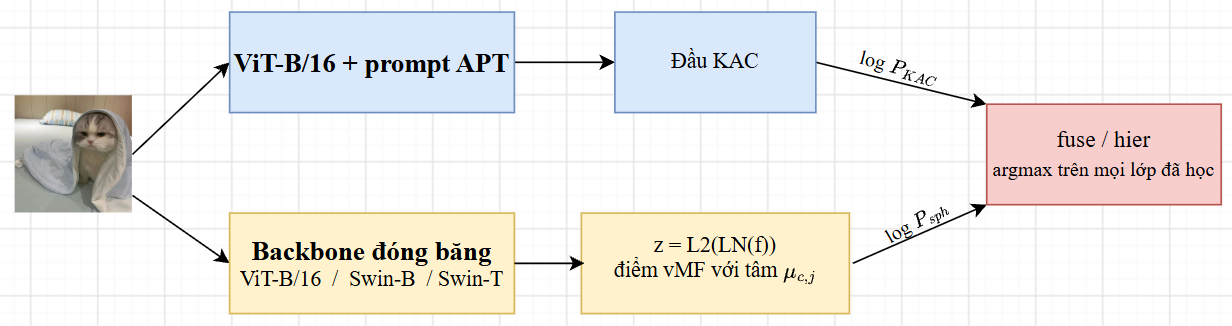
\includegraphics[width=\linewidth]{hinh1.png}
\caption{Sơ đồ APT + KAC + nhánh Spherical. Nhánh trên (xanh) giữ nguyên Baseline. Nhánh dưới (cam) là phần thêm vào: một lượt forward qua backbone đóng băng, không huấn luyện thêm tham số nào. Với nguồn APT (stale/refresh), nhánh dưới dùng chính đặc trưng của nhánh trên.}
\end{figure}

\subsection{Vấn đề của KAC khi không biết task id}
Ở task $t$, KAC chỉ được huấn luyện bằng cross-entropy trên các lớp của task $t$:
\begin{equation}
\mathcal{L}_t = -\log \frac{\exp(\ell_y)}{\sum_{j \in B_t} \exp(\ell_j)}.
\end{equation}
Loss này không đổi nếu cộng cùng một hằng số $b_t$ vào mọi logit của khối $B_t$. Vì vậy mức nền của mỗi khối là tùy ý: không có gì buộc logit của task 3 và task 7 nằm trên cùng một thang. Khi suy luận lấy $\arg\max_{c}\ell_c$ trên mọi lớp đã học, một khối có mức nền cao sẽ ``hút'' dự đoán, dù lớp đúng nằm ở khối khác. Vì vậy lỗi chủ yếu nằm ở bước chọn task, không phải ở việc phân biệt lớp trong cùng task.

\subsection{Nhánh Spherical}
\textbf{Đặc trưng trên mặt cầu.} Với đặc trưng $f$ từ nguồn đã chọn, $z = \mathrm{L2}\big(\mathrm{LayerNorm}(f)\big)$, tức $\|z\|=1$.

\textbf{Tâm lớp.} Với mỗi lớp $c$, chạy spherical k-means (20 vòng) trên đặc trưng train của lớp đó, thu được $k$ tâm $\mu_{c,1},\dots,\mu_{c,k}$ ($\|\mu_{c,j}\|=1$). Tâm được tính một lần khi học task chứa lớp $c$, sau đó không cần ảnh cũ nữa.

\textbf{Điểm vMF.} Điểm của lớp $c$ là log-tổng các thành phần vMF:
\begin{equation}
s_c(z) = \log \sum_{j=1}^{k} \exp\!\big(\kappa\,(z^\top \mu_{c,j} - 1)\big), \qquad
\kappa = \frac{\kappa_{mult}}{\operatorname{median}_{i<j}\big(1 - z_i^\top z_j\big)},
\end{equation}
trong đó median lấy trên các cặp đặc trưng train, để $\kappa$ tự thích nghi với độ phân tán của từng dataset. $P_{sph}(c\mid x) = \operatorname{softmax}_c\big(s_c(z)\big)$ trên mọi lớp đã học. Vì mọi tâm nằm trên cùng mặt cầu và dùng chung $\kappa$, điểm của các task khác nhau \emph{so sánh được trực tiếp}. Đây chính là điều KAC còn thiếu.

\textbf{Biến thể \texttt{fuse}.}
\begin{equation}
\label{eq:fuse}
\hat y = \arg\max_c \Big[(1-w)\log P_{KAC}(c\mid x) + w \log P_{sph}(c\mid x)\Big].
\end{equation}

\textbf{Biến thể \texttt{hier}.} Spherical cho xác suất task $\log P_{sph}(t\mid x) = \operatorname{logsumexp}_{c\in B_t}\log P_{sph}(c\mid x)$. Trong task, dùng log-softmax theo khối của KAC và của Spherical:
\begin{equation}
\label{eq:hier}
\hat y = \arg\max_c \Big[\lambda \log P_{sph}(t(c)\mid x) + (1-w_{in})\log P^{B}_{KAC}(c\mid x) + w_{in}\log P^{B}_{sph}(c\mid x)\Big].
\end{equation}

\textbf{Lưới siêu tham số:} $k\in\{1,3,5\}$, $\kappa_{mult}\in\{8,16,32,64\}$, $w\in\{0.25,0.5,0.75\}$, $\lambda\in\{0.5,1,2\}$, $w_{in}\in\{0,0.5\}$. Nhánh Spherical không có tham số học bằng gradient.

\subsection{Các điểm thảo luận}
\begin{enumerate}
  \item \textbf{\texttt{fuse} ổn định hơn \texttt{hier}.} \texttt{fuse} cho Last cao hơn \texttt{hier} ở 17/20 ô. \texttt{hier} chỉ nhỉnh hơn khi nhánh Spherical đã rất mạnh (CUB-200 với ViT-B/16: 84.97 so với 84.89; APT refresh trên CIFAR-100 và CUB-200), và Forgetting của \texttt{hier} cao hơn ở 19/20 ô. Lý do: \texttt{hier} để Spherical quyết định task một cách cứng, nên khi Spherical chọn sai task thì KAC không sửa lại được. \texttt{fuse} cho hai nhánh bù lỗi cho nhau.
  \item \textbf{Drift của đặc trưng APT.} APT (stale) tốt hơn Baseline nhưng kém ViT-B/16 đóng băng trên CUB-200 (79.28 so với 84.89) và Stanford Cars, đồng thời Forgetting tăng mạnh (CUB-200: 14.48 so với 5.49). Nguyên nhân là prompt tiếp tục được cập nhật sau mỗi task, nên đặc trưng của ảnh cũ dịch chuyển khỏi tâm đã lưu. Khi tính lại tâm bằng mô hình hiện tại (refresh, Tham chiếu), CUB-200 lên 85.94 và Stanford Cars lên 69.06, cao nhất trong bảng. Như vậy đặc trưng APT có tiềm năng tốt hơn, nếu bù được drift mà không cần ảnh cũ.
  \item \textbf{Chọn backbone.} ViT-B/16 đóng băng là lựa chọn cân bằng nhất: không thêm tham số và mức tăng gần bằng Swin-B. Swin-B chỉ hơn $0.1$--$1.1$ điểm nhưng nặng và chậm hơn. Swin-T rẻ nhất nhưng tụt rõ trên CUB-200.
  \item \textbf{Siêu tham số được chọn.} $k\in\{3,5\}$ thường tốt nhất trên CIFAR-100, ImageNet-R và Stanford Cars (lớp đa dạng, nhiều cụm). Trên CUB-200 với ViT-B/16, $k=1$ và $\kappa_{mult}$ lớn (64) tốt nhất, phù hợp với dataset ít ảnh mỗi lớp ($\sim$24 ảnh train/lớp sau khi tách Val).
\end{enumerate}

\section{Hạn Chế và Hướng Tiếp Theo}
\begin{itemize}
  \item \textbf{Chỉ có số liệu Val.} Cấu hình được chọn trên chính Val, nên số liệu có thể lạc quan. Bước tiếp theo là chốt một cấu hình cho mỗi dataset (đề xuất \texttt{fuse} + ViT-B/16 đóng băng) và chạy tập Test một lần.
  \item \textbf{Chi phí suy luận gấp đôi} do lượt forward thứ hai. Hướng tiếp theo là dùng đặc trưng APT cho nhánh Spherical và bù drift bằng Semantic Drift Compensation (ước lượng độ dịch của tâm cũ từ độ dịch của đặc trưng dữ liệu mới), để bỏ lượt forward thứ hai mà vẫn tiến gần mức APT (refresh).
  \item \textbf{Stanford Cars dao động lớn giữa các seed}, cần thêm seed hoặc số liệu Test trước khi kết luận về mức tăng trên dataset này.
\end{itemize}

\section{Phụ Lục}
\subsection*{Phụ lục A: Siêu tham số huấn luyện APT + KAC (dùng chung cho Baseline và Ours)}
\begin{table}[H]
\centering\small
\begin{tabular}{lcccc}
\toprule
Siêu tham số & CIFAR-100 & CUB-200 & Stanford Cars & ImageNet-R \\
\midrule
Learning rate (prompt) & 0.004 & 0.02 & 0.005 & 0.003 \\
Số epoch & 30 & 25 & 50 & 30 \\
Hệ số EMA & 0.7 & 0.7 & 0.7 & 0.8 \\
Batch size & 64 & 64 & 64 & 64 \\
\texttt{prompt\_param} & 0.01 & 0.01 & 0.01 & 0.01 \\
Đầu KAC & \multicolumn{4}{c}{4 lưới RBF, lr head $10^{-3}$} \\
Optimizer / lịch LR & \multicolumn{4}{c}{Adam, cosine (theo repo APT)} \\
\bottomrule
\end{tabular}
\end{table}

\subsection*{Phụ lục B: Last theo từng seed}
Kiểm tra độ ổn định. Trung bình của 3 seed khớp với Bảng 2. Bảng này chỉ gồm Baseline và các nguồn đóng băng. Số liệu theo seed của APT (stale/refresh) nằm trong file kết quả gốc.

{\small
\setlength{\tabcolsep}{5pt}
\begin{longtable}{lllcccc}
\caption{\textbf{Bảng B:} Last (\%) theo seed [Tập Validation]}\\
\toprule
Dataset & Phương pháp & Biến thể & Seed 0 & Seed 1 & Seed 2 & TB $\pm$ ĐLC \\
\midrule
\endfirsthead
\toprule
Dataset & Phương pháp & Biến thể & Seed 0 & Seed 1 & Seed 2 & TB $\pm$ ĐLC \\
\midrule
\endhead
\bottomrule
\endfoot
\multirow{7}{*}{CIFAR-100} & APT + KAC & -- & 88.84 & 87.53 & 87.66 & 88.01 $\pm$ 0.72 \\
 & ViT-B/16 đóng băng & fuse & 89.77 & 88.75 & 88.71 & 89.08 $\pm$ 0.60 \\
 & ViT-B/16 đóng băng & hier & 85.38 & 85.07 & 84.58 & 85.01 $\pm$ 0.40 \\
 & Swin-B đóng băng & fuse & 90.39 & 89.84 & 89.25 & 89.83 $\pm$ 0.57 \\
 & Swin-B đóng băng & hier & 87.22 & 87.83 & 86.81 & 87.29 $\pm$ 0.51 \\
 & Swin-T đóng băng & fuse & 89.34 & 88.24 & 88.34 & 88.64 $\pm$ 0.61 \\
 & Swin-T đóng băng & hier & 79.23 & 80.27 & 79.74 & 79.75 $\pm$ 0.52 \\
\midrule
\multirow{7}{*}{CUB-200} & APT + KAC & -- & 75.92 & 75.17 & 76.75 & 75.94 $\pm$ 0.79 \\
 & ViT-B/16 đóng băng & fuse & 84.17 & 84.67 & 85.83 & 84.89 $\pm$ 0.86 \\
 & ViT-B/16 đóng băng & hier & 84.25 & 84.75 & 85.92 & 84.97 $\pm$ 0.86 \\
 & Swin-B đóng băng & fuse & 84.50 & 84.75 & 85.75 & 85.00 $\pm$ 0.66 \\
 & Swin-B đóng băng & hier & 83.92 & 84.08 & 83.58 & 83.86 $\pm$ 0.25 \\
 & Swin-T đóng băng & fuse & 79.58 & 79.25 & 80.42 & 79.75 $\pm$ 0.60 \\
 & Swin-T đóng băng & hier & 70.58 & 70.58 & 69.75 & 70.31 $\pm$ 0.48 \\
\midrule
\multirow{7}{*}{Stanford Cars} & APT + KAC & -- & 65.91 & 64.90 & 58.60 & 63.14 $\pm$ 3.96 \\
 & ViT-B/16 đóng băng & fuse & 66.51 & 66.70 & 62.10 & 65.10 $\pm$ 2.61 \\
 & ViT-B/16 đóng băng & hier & 59.14 & 56.15 & 58.56 & 57.95 $\pm$ 1.59 \\
 & Swin-B đóng băng & fuse & 67.22 & 66.76 & 62.52 & 65.50 $\pm$ 2.59 \\
 & Swin-B đóng băng & hier & 57.72 & 56.83 & 58.99 & 57.85 $\pm$ 1.09 \\
 & Swin-T đóng băng & fuse & 66.16 & 66.28 & 61.76 & 64.73 $\pm$ 2.57 \\
 & Swin-T đóng băng & hier & 55.70 & 54.46 & 53.80 & 54.65 $\pm$ 0.97 \\
\midrule
\multirow{7}{*}{ImageNet-R} & APT + KAC & -- & 77.82 & 78.39 & 77.52 & 77.91 $\pm$ 0.44 \\
 & ViT-B/16 đóng băng & fuse & 78.58 & 78.43 & 78.39 & 78.47 $\pm$ 0.10 \\
 & ViT-B/16 đóng băng & hier & 76.05 & 76.26 & 76.07 & 76.13 $\pm$ 0.11 \\
 & Swin-B đóng băng & fuse & 79.58 & 79.66 & 79.36 & 79.54 $\pm$ 0.15 \\
 & Swin-B đóng băng & hier & 76.83 & 77.20 & 76.87 & 76.97 $\pm$ 0.21 \\
 & Swin-T đóng băng & fuse & 78.51 & 78.71 & 78.49 & 78.57 $\pm$ 0.12 \\
 & Swin-T đóng băng & hier & 74.12 & 74.59 & 74.20 & 74.30 $\pm$ 0.25 \\
\end{longtable}
}

\end{document}
